%*****************************************************************************
	\chapter{Analysis and design of the solution}
	Based on the assignment I was asking a question \emph{How should the dialogue with a blind pedestrian look like?} After hours spent thinking about how to do it. I was advised from my supervisor just to observe. So I did. I used an iterative technique, where I started analysing dialogue of two people and ended up with a fully standalone web app.
	
	I did five iterations, tested them and implemented the outputs of one iteration to a next iteration.
	
	In the first iteration was just talking with users and try to localize them on a map.
	
	In the second iteration a I was controlling a computer which talked to the users in a machine voice and the people talked back to me.
	
	In the third iteration I improved the previous prototype and tested it in the city.
	
	In the fourth iteration branched for two directions. First direction asking user about the address, street and or public transport stops. Second direction using heavily GPS, guiding user around a corner of a street and matching his path to map data.
	
	In the fifth iteration I put the most promising methods of the fourth iteration to a code and validated how they succeedd while using by real users (blinds) in real environment (city).
	
	The whole developement focused on usage in the center of Prague.
	\section{Iteration 1 - talking}
	\label{sec:FirstExperiment}
	
	\begin{labeling}{number of prototypes}
		\item [people] sighted
		\item [environment] map
		\item [number of prototypes] 1
		\item [implementation] none
	\end{labeling}
	
	I started with a game. Two player game, one player was simulating a \emph{\uv{blind} user} walking in a city the second player was seeker. I was playing the \emph{seeker}, asking the user questions and trying to localize him.
	
	%todo image
	\begin{figure}[h]
		\centering
		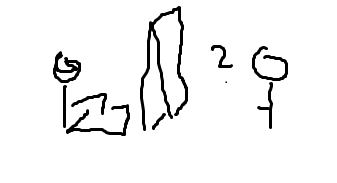
\includegraphics[width=0.7\linewidth]{figures/1stExp-human2humanOverMap/bigpicture}
		\caption[Setup]{}
		\caption{}
		\label{fig:bigpicture}
	\end{figure}

	These game sessions were recorded and then analysed. The analysis shown the \emph{topics} and \emph{questions}, which was repeating. And could be used for an automated dialogue system.
	
	
	\paragraph{\uv{blind} user}
	The user was given the map and a piece of paper with cut out hole. See \ref{fig:map-and-blind-simulator}. The map was depicting all the enviroment: inclination of sidewalks, pedestrian crossings,  marking for blinds, rails, houses, parked cars, noises form cars, ticking noises from trafic lights, direction of cars, tram lines.
	
	The user choosed a place on a side walk he liked and put a cut out hole on that spot. Then he was responding the seekers questions, moving and exploring the environment based on seekers orders.
	
	\paragraph{seeker}
	The seeker had another copy of the map. He was asking the \emph{\uv{blind} user} questions and giving him orders. \uv{Do you have there buildings?}, \uv{Which hands do you have the house on?}, \uv{Are you going up hill?}. 
	Depending on the response i.e \uv{I am going downhill.} He was eliminating all the not suitable places (uphills, and horizontal sidewalks). When the possible space on the sidewalks narrowed to one point the seeker anouced \uv{Found you, you are here!} and showed it to the \uv{blind} user.
	
	\begin{figure}[h]
		\centering
		\includegraphics[width=0.7\linewidth]{"figures/1stExp-human2humanOverMap/map and blind simulator"}
		\caption[Map and blind simulator]{A map and paper with cutout hole, to simulate blind person and space he can explore}
		\label{fig:map-and-blind-simulator}
	\end{figure}
	\begin{figure}[h]
		\centering
		\includegraphics[width=0.7\linewidth]{"figures/1stExp-human2humanOverMap/using blind simulator"}
		\caption[User session]{A user is moving on the map and answering the questions of the facilitator}
		\label{fig:user-session}
	\end{figure}
	
	\paragraph{outputs}
	I was collecting all the answers the \emph{seeker} used. Then I clustered these questions accroding the topic and selected the most representative answer for each topic.
	
	\paragraph{testing details}
	Five friends interacted as users in this study. 3 mens and 2 womens. They were between 21 and 53 years old. Each participant went over 4 maps with consequently growing complexity of the environment.

	
	
	
	%todo picture of questions and answer
	\begin{figure}[h]
		\centering
		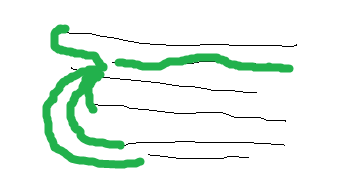
\includegraphics[width=0.7\linewidth]{figures/1stExp-human2humanOverMap/clusteredquestions}
		\caption[Best question for each topic]{}
		\caption{}
		\label{fig:clusteredquestions}
	\end{figure}
	
	The topics and the questions were
	\begin{itemize}
		\item \emph{Orders} - Describe where you are? Is there anything else interesting?
		\item \emph{Houses} - Do you have houses?
		\item ...
		%todo complete list
	\end{itemize}
	
		
	\section{Iteration 2 - dialogue system}
	\begin{labeling}{number of prototypes}
		\item [people] sighted
		\item [environment] map
		\item [number of prototypes] 1
		\item [implementation] Wizard of Oz
	\end{labeling}
	As a second step I built a low fidelity prototype of dialogue system. I wanted to verify the questions from the first experiment would work even when read aloud by a computer system and to see how the interaction would change.
	
	 I used Axure\cite{axure} to create a diagram and craft the logic of this system. And I used the Accapela text to speech (TTS) service\cite{accapela} to prerecord all seeker's questions and possible answers. So whenever I clicked on a field in the diagram, the computer read it alloud.
	 
	  I repeated the game from the first experiment, but this time the seeker was asking his questions based on the diagram logic, and as a response clicking on correct answer and leting it be read aloud by the machine voice.
	 
	 %todo fix images dialogue + largerimage of dialogue
\begin{figure*}[h]
	\centering
	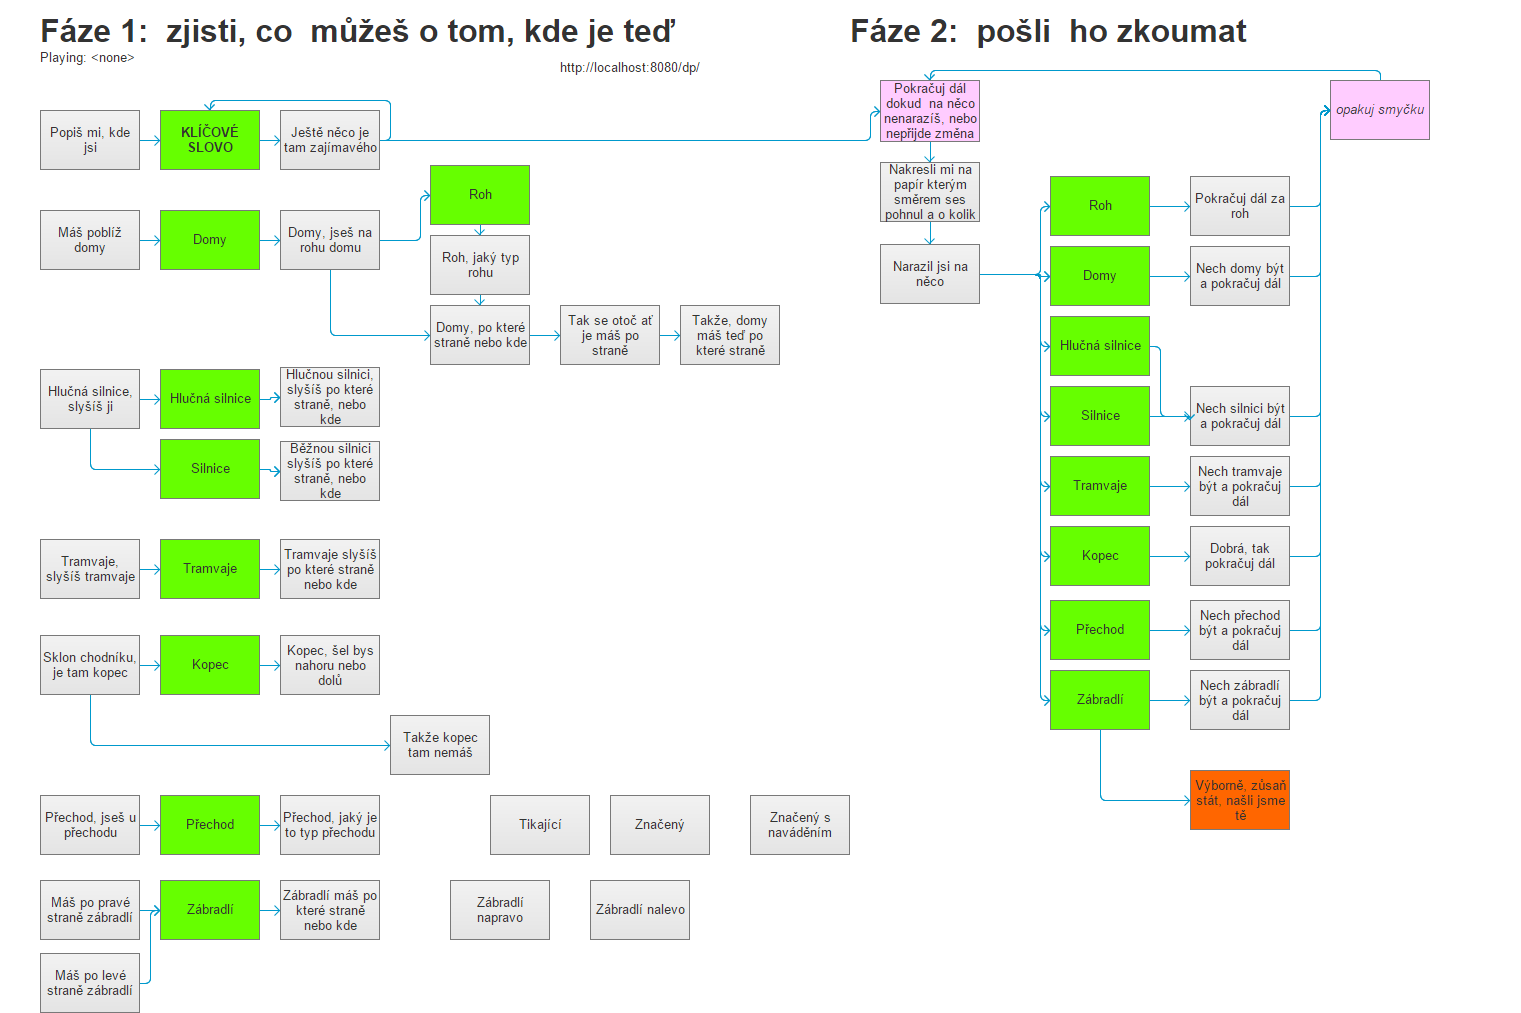
\includegraphics[width=0.7\linewidth]{figures/2ndExp-human2WoZOverMap/tested-dialogue}
	\caption[Dialogue]{}
	\caption{}
	\label{fig:tested-dialogue}
\end{figure*}


\begin{figure}[h]
	\centering
	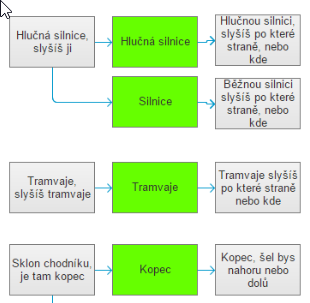
\includegraphics[width=0.7\linewidth]{figures/2ndExp-human2WoZOverMap/detail}
	\caption[Detail]{}
	\caption{}
	\label{fig:detail}
\end{figure}

\paragraph{outcomes}
I noticed the participants started to talk a lot woth one world setneces like \uv{yes}, \uv{uphill} or at least make very short senteces. All the richness of ansewers disappeared and the answers started to be very similiar between the participants. So when someone would give you the anonymised transcript, you could even recognize if it is from one person or not.
Next I evaluated the usability and comed up with a list of usability mistakes and errors in the possible ansers and minor dialogue issue in structure.

\paragraph{participants}
Another set of 5 friends of mine participated. Their age ranged from ? to ?. ? mens and ? womens. They again went as wall throught the same 4 maps with increasing complexity

	
	 I 
	\section{Iteration 3 - fixed dialogue system}
	\begin{labeling}{number of prototypes}
		\item [people] sighted
		\item [environment] city
		\item [number of prototypes] 1
		\item [implementation] Wizard of Oz
	\end{labeling}
	\section{Iteration 4 - new variants}
	\begin{labeling}{number of prototypes}
		\item [people] blind
		\item [environment] city
		\item [number of prototypes] 5
		\item [implementation] Wizard of Oz
	\end{labeling}
	From the second and thir experiment I learned that it's sometimes impossible to decide the possition of person, it takes long and is error prone. And as well I compared it with the Naviterier data structure \cite{naviterier-data}. 
	%todo how it was exactly, what do i need
	I realised that most of the needed infos like trams, type of corners, altitude are not present in the API, thus not able to be used in a standallone application.
	
	And I started to play with Idea, do we even need it, can we just smartly use the data from the GPS, or utilize a person just hopped of the tram he knows the number and knows the stop?
	
	I came up with five prototypes. 
	
	\paragraph{POI}
	\paragraph{POI - with GPS}
	\paragraph{Crossing of two streets}
	\paragraph{GPS \& compass}
	\paragraph{GPS wo compass}
	
	
	This time the Wizzard of Oz simulation went even further. The user was given a phone. And instructed, when he taps the upper part of the screen it means button one, lower part means button two. In fact the phone was turned off. The researcher was standing nearby and determining the dialog again by clicking and letting the computer read aloud the TTS texts.
	
	\paragraph{outputs}
	
	%todo see https://docs.google.com/document/d/1xfWjAOKCVGUYHrUM910tLNwEvJqrzqakL6JYwVVPzdc/edit
	
	
	 
	\section{Iteration 5 - fixed variants}
	\begin{labeling}{number of prototypes}
		\item [people] blind
		\item [environment] city
		\item [number of prototypes] 3
		\item [implementation] Website + backend
	\end{labeling}

	The last iteration brought three prototypes: \reversegeo, \gps and \poi. All three of them are fully working. The users can interact with them in the browser.
		
	
	\paragraph{\reversegeo}
	\reversegeo prototype uses user's current position. The GPS senstor in the phone tells the user's coordinates: latitude and longitude. The HERE API \cite{here-api} estimates what is the nearest address for user's coordinates. Parallel to that the prototype asks user for the address he want's to go. And then finaly the navigation is started between the estimated address and the address user wants to go.
	
	%todo screens
	
	I expected the \reversegeo would fail in case the nearest address would be on the opposite sidewalk accross the street. But it should demonstrate the state-of-the-art solution. Since it uses only currently used technologies. 
	
	
	\paragraph{\poi}
	\poi prototype simulates a dialogue. The system asks question and the user can respond as he will. The answer is sent to Conversational API\cite{conversational-api} from IBM. Which can uderstand the context and infromation the user said.
	
	The \poi asks for address user want to go and then ask user for current position, where he stands. The current positioncan be the address or the name of the tramstop. When some information is not complete, the system asks the follow up questions.
	
	Let's say the user wants to go to Myslíkova 22, and arrived by the tram 9 to Národní třída. The tram disapeared in the direction Národní Divadlo. And the user is on the stop platform. The dialogue then can look like:
	
	Wellcome my friend, where are you going? 
	Myslíkova 22
	You are going to Myslíkova 22. What is your current address, or what is your public transport stop?
	Tram Narodní Třída.
	You are on stop Národní třída. Let's determine exact platform. What line and in which direction? (next stop is sufficent info)
	9 Národní divadlo
	So you are now leaving from stop Národní třída, line 9 in direction Národní divadlo.
	
	Or
	
	
	Wellcome my friend, where are you going? 
	Myslíkova
	You are going to Myslíkova, What is the house number?
	22
	You are going to Myslíkova 22. What is your current address, or what is your public transport stop?
	Národní Třída.
	Not sure, Did you meant street Národní or stop Národní třída?
	Stop
	You are on stop Národní třída. Let's determine exact platform. What line and in which direction? (next stop is sufficent info)
	9
	Line 9. In which direction? (next stop is sufficient info)
	... and so on
	
	
	
	In both cases it will extract the parameters
	\begin{itemize}
		\item target street: Myslíkova
		\item target house number: 22
		\item source line: 9
		\item source stop name: Národní třída
		\item source next stop: Národní divadlo
	\end{itemize}

	The triplet (line, stop name, next stop) is converted to GPS coordinates and these GPS coordinates to an address. This address is then used as source address to launch navigation from target address to this source address.
	
	Triplet to GPS coords: DPP API (described in section \ref{triplet-api})
	GPS coords to address: HERE API \cite{here-api}
	User input to meaning: Conversational API from IBM \cite{conversational-api}
	
	%img of prototype
		
	
	\paragraph{\gps}
	The \gps sends the user in correct direction, collects his coordintates on the way and then tries to estimate the best position on the sidewalk.
	
	\gps asks for the address of the target. Then users stands with his backs to the wall. The compass built in the phone tells which direction is the shortest air-path to the target. if it is in interval <90\degree, -90\degree> it sends him right in (90\degree, 270\degree) sends him left
	
	%img where send left when right
	\begin{figure}
		\centering
		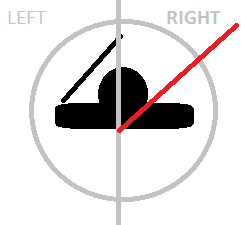
\includegraphics[width=0.7\linewidth]{figures/5thExp-blind2phoneInCity/gps-gorightorgoleft}
		\caption{}
		\label{fig:gps-gorightorgoleft}
	\end{figure}
	
	
	Then it starts coolecting coordinates. The user goes to the side (in this example right) and goes to the corner of the building. He mark down to the app he is on the corner. And walks another cca 30 meters. Then he hits estimate my position. His logged coordinates are matched to the map of sidewalks in Naviterier maps \cite{naviterier-maps}. Then the app knows which sidewalk he is standig on. Next the app projects his current gps coordinates to the nearest position on sidewalk.
	
	From this sidewalk the app just finds the nearest address on this given sidewalk and starts a navigation from this point.
	
	%img process of walking, matching, estimate sidewalk, estimate projection, estimate address
	
	%img screens
	
	Coordinates on sidewalk to address: GPS address api (described in \ref{gps-address-api})
	
	
	\paragraph{restrictions}
	I needed to keep the complexity reduced for the prototyping. The goal of these prototypes was to validate the idea works. I was not interested in covering the whole problem of point to point navigation.
	The further systems could accept as well points of interest ie "pizza restaurant in Lazarská" and stops of all means of public transport (buses, metro, trains).
	Since the point of the interests can be decoded to GPS coordinates using i.e. Google API \cite{google-api}. And the data about other means of public transport are covered in the open DPP data \cite{dpp-data} and I could use the same algorithm as for trams.
	
	In the \gps prototype to speed up the protyping cyclus I didn't make the algorithm perfect. As well I didn't validate if there is the map data for given area. The testing will be done in area, which is covered and again I am going to validate the idea is working, not to deliver full experience.
	
	